\documentclass[12pt,a4paper]{article}
\usepackage[UTF8]{ctex}
\usepackage{graphicx}
\usepackage{geometry}
\usepackage{ulem}
\usepackage{enumitem}
\usepackage{titlesec}
\usepackage{multicol}
\usepackage[export]{adjustbox}
\usepackage{amsmath}  % 推荐用于更好的数学排版
\usepackage[utf8]{inputenc}
\usepackage{CJKutf8}
\usepackage{fancyhdr}
\usepackage{lastpage}
\usepackage{tabularx}
\usepackage{float}
\usepackage{siunitx}
\usepackage{multirow} 

% 页眉页脚设置
\pagestyle{fancy}
\fancyhf{} % 清除所有页眉页脚
% 设置页眉内容
\fancyhead[C]{\small
    \makebox[4.5em][c]{实验名称：} \uline{\makebox[17em][c]{天线CST仿真}} 
    \makebox[2.5em][c]{姓名：} \uline{\makebox[4em][c]{张赫}} 
    \makebox[2.5em][c]{学号：} \uline{\makebox[5em][c]{3240101459}}
}
\fancyfoot[C]{\small 第 \thepage\ 页，共 \pageref{LastPage} 页}

% 取消页眉和页脚的下划线
\renewcommand{\headrulewidth}{0pt}
\renewcommand{\footrulewidth}{0pt}

% 调整页眉高度
\setlength{\headheight}{50pt}

% 设置plain样式（用于第一页）
\fancypagestyle{plain}{
    \fancyhf{}
    \renewcommand{\headrulewidth}{0pt}
    \fancyfoot[C]{第 \thepage\ 页，共 \pageref{LastPage} 页}
}

% 设置页面边距
\geometry{left=2.54cm,right=1.5cm,top=2.54cm,bottom=2.54cm}

% 设置正文字体大小为小四
\renewcommand{\normalsize}{\fontsize{12pt}{16pt}\selectfont}

% 设置章节格式
\titleformat{\section}{\fontsize{16pt}{22pt}\selectfont\bfseries}{\thesection}{1em}{}
\titleformat{\subsection}{\fontsize{15pt}{20pt}\selectfont\bfseries}{\thesubsection}{1em}{}
\titleformat{\subsubsection}{\fontsize{14pt}{18pt}\selectfont\bfseries}{\thesubsubsection}{1em}{}

\begin{document}

\thispagestyle{plain}

% 标题部分 - 两栏布局
\begin{multicols}{2}
    % 左栏：图片和实验报告标题
    \noindent
    ~\\ % 第一行
    ~\\ % 第二行
    ~\\ % 第三行
    \hphantom{占位}
    \raisebox{-0.5\baselineskip}
    {
\includegraphics[width=1.85in,height=0.58in]{ZJU.jpg}}
    \hspace{.5em}
    \raisebox{0pt}[\height][0pt]
    {\textbf{\fontsize{26pt}{30pt}\selectfont 实验报告}}
    
    \columnbreak
    
    % 右栏：个人信息
    \begin{flushright}
        \small
        \makebox[3em][l]{专业：} \uline{\makebox[9em][c]{法语-电子科学与技术}} \\
        \makebox[3em][l]{姓名：} \uline{\makebox[9em][c]{张赫}} \\
        \makebox[3em][l]{学号：} \uline{\makebox[9em][c]{3240101459}} \\
        \makebox[3em][l]{日期：} \uline{\makebox[9em][c]{2026年4月17日}} \\
        \makebox[3em][l]{地点：} \uline{\makebox[9em][c]{}} \\
    \end{flushright}   
\end{multicols}

% 课程名称等信息
{\small
\noindent
课程名称： \uline{电磁场与电磁波} \hfill 指导老师： \uline{李凯、王子立} \hfill 成绩： \uline{\hspace{3cm}} \\
实验名称：\uline{天线CST仿真}\hfill 实验类型：\uline{验证实验}\hfill 同组学生姓名：\uline{}
}

\section*{一、实验过程}

\subsection*{1 建立模型}

\subsubsection*{创建参数}
如下图所示新增参数。

\begin{figure}[H]
    \centering
    
\includegraphics[width=0.8\textwidth]{1.png}
\end{figure}

\subsubsection*{创建波导}
Modeling选项卡 $\Rightarrow$ Shape栏目 $\Rightarrow$ brick图标，按如下参数创建矩形波导。

\begin{figure}[H]
    \centering
    
\includegraphics[width=0.4\textwidth]{2.png}
\end{figure}

\begin{figure}[H]
    \centering
    
\includegraphics[width=0.4\textwidth]{3.png}
\end{figure}

\subsubsection*{创建喇叭口径面}
Modeling选项卡 $\Rightarrow$ Curves栏目 $\Rightarrow$ Curves $\Rightarrow$ Rectangle，按如下参数创建喇叭口径面。

\begin{figure}[H]
    \centering
    
\includegraphics[width=0.4\textwidth]{4.png}
\end{figure}

Modeling选项卡 $\Rightarrow$ Shape栏目 $\Rightarrow$ Create Shape from Curve $\Rightarrow$ Cover Curve

\subsubsection*{设置喇叭口径面的空间位置}
先 Modeling选项卡 $\Rightarrow$ Picks栏目 $\Rightarrow$ Pick Face选中口径面，然后 Modeling选项卡 $\Rightarrow$ Tools栏目 $\Rightarrow$ Transform $\Rightarrow$ Translate设置口径面的位置（Translation Vector，Z设置为$-L$）。

\begin{figure}[H]
    \centering
    
\includegraphics[width=0.6\textwidth]{5.png}
\end{figure}

\subsubsection*{创建喇叭侧壁}
分别选中波导和喇叭的口径面，Modeling选项卡 $\Rightarrow$ Shape栏目 $\Rightarrow$ Loft图标，创建天线的侧壁。

\begin{figure}[H]
    \centering
    
\includegraphics[width=0.4\textwidth]{6.png}
\end{figure}

\begin{figure}[H]
    \centering
    
\includegraphics[width=0.6\textwidth]{7.png}
\end{figure}

\subsubsection*{全层相加}
Modeling选项卡 $\Rightarrow$ Tools栏目 $\Rightarrow$ Boolean $\Rightarrow$ Add把整个PEC层变成一个整体。

\subsubsection*{掏空}
分别选取天线前后两个面，然后Modeling选项卡 $\Rightarrow$ Tools栏目 $\Rightarrow$ Shape Tools $\Rightarrow$ Shell Solid or Thicken Sheet掏空生成喇叭。

\begin{figure}[H]
    \centering
    
\includegraphics[width=0.4\textwidth]{8.png}
\end{figure}

\begin{figure}[H]
    \centering
    
\includegraphics[width=0.6\textwidth]{9.png}
\end{figure}

至此我们便完成了天线的建模。

\subsection*{2 仿真}

\subsubsection*{设置仿真频率}
Simulation选项卡 $\Rightarrow$ Setting栏目 $\Rightarrow$ Frequency设置仿真频率（8.2GHz $\sim$ 12.4GHz）。

\begin{figure}[H]
    \centering
    
\includegraphics[width=0.4\textwidth]{10.png}
\end{figure}

\subsubsection*{设置仿真边界条件}
Simulation选项卡 $\Rightarrow$ Setting栏目 $\Rightarrow$ Background设置为Normal。

\begin{figure}[H]
    \centering
    
\includegraphics[width=0.4\textwidth]{11.png}
\end{figure}

Simulation选项卡 $\Rightarrow$ Setting栏目 $\Rightarrow$ Boundaries设置为 open (add space)。

\begin{figure}[H]
    \centering
    
\includegraphics[width=0.5\textwidth]{12.png}
\end{figure}

\subsubsection*{端口设置}
Modeling选项卡 $\Rightarrow$ Picks栏目 $\Rightarrow$ Pick Face设置波导端口。

然后 Simulation选项卡 $\Rightarrow$ Source and Load栏目 $\Rightarrow$ Waveguide Ports确定模式吸收数（Number of modes = 5）。

\subsubsection*{设置监视器}
Simulation选项卡 $\Rightarrow$ Monitor栏目 $\Rightarrow$ Field Monitor设置type为Farfield（RCS），中心频率为10.3GHz。

\begin{figure}[H]
    \centering
    
\includegraphics[width=0.4\textwidth]{13.png}
\end{figure}

\section*{二、实验数据记录}

\subsection*{喇叭天线S11曲线}
\begin{figure}[H]
    \centering
    
\includegraphics[width=1.0\textwidth]{14.png}
\end{figure}

从仿真得到的 S11 曲线可以看出，在 8.2–12.4 GHz 的工作频段内，天线的反射系数 S11 整体低于 -20 dB，在 9.5–11.5 GHz 范围内甚至低于 -40 dB，最低点达到约 -52 dB（位于 10.2 GHz 附近）。

这表明：
\begin{itemize}
    \item 天线与馈电波导之间实现了良好的阻抗匹配，馈入的能量绝大部分由喇叭口辐射出去，反射能量极少。
    \item S11 $< -20$ dB 通常被认为是工程上“优良匹配”的标准，本天线完全满足。
\end{itemize}

\subsection*{喇叭天线驻波比特性曲线}
\begin{figure}[H]
    \centering
    
\includegraphics[width=1.0\textwidth]{15.png}
\end{figure}

S11 与 VSWR 是一一对应的关系。S11 = -20 dB 对应 VSWR $\approx$ 1.22，S11 = -40 dB 对应 VSWR $\approx$ 1.02。因此，本天线在整个工作频段内的 VSWR 均小于 1.22，在最佳频点处接近 1，说明匹配性能优异。

\textbf{与理论预期对比：}

由于本实验采用的喇叭尺寸较标准 X 波段喇叭偏小，其最佳匹配频点出现在 10.2 GHz，较中心频率 10.3 GHz 略有偏高，符合天线理论中“尺寸减小会导致工作频率升高”的规律。

\subsection*{喇叭天线水平方向图}
\begin{figure}[H]
    \centering
    
\includegraphics[width=0.6\textwidth]{16.png}
\end{figure}

\textbf{水平方向图分析（H面，$\phi = 0^\circ$）：}

H面方向图主瓣指向 $0^\circ$ 方向，3dB波束宽度约为 $55^\circ$-$60^\circ$，呈现出良好的对称性。副瓣电平约为 -13 dB。

\subsection*{喇叭天线垂直方向图}
\begin{figure}[H]
    \centering
    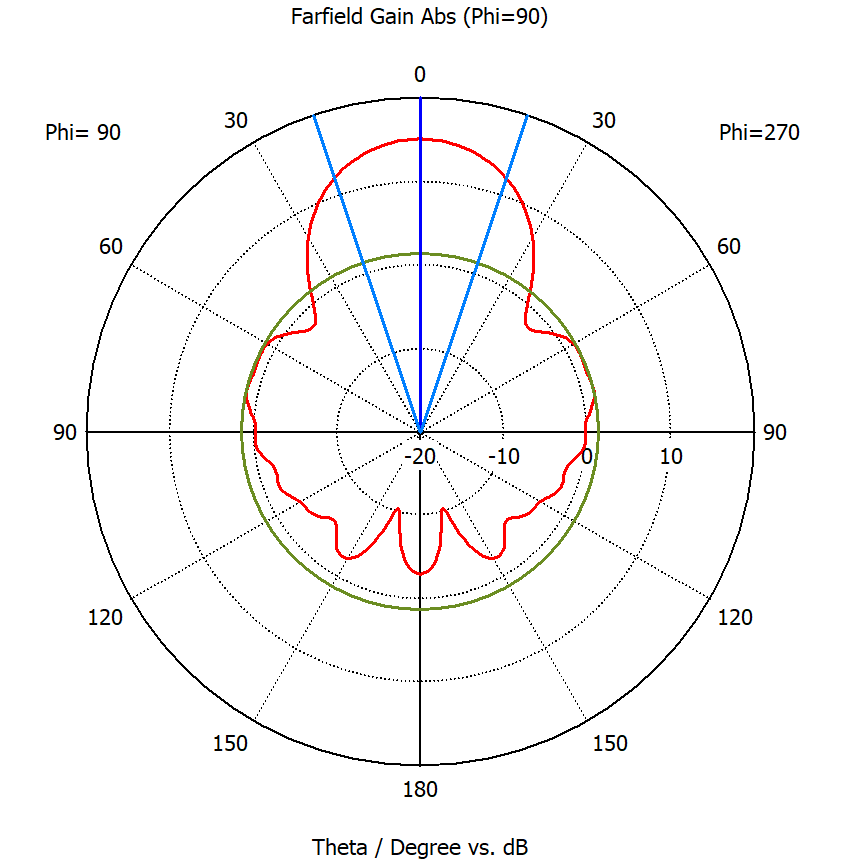
\includegraphics[width=0.6\textwidth]{17.png}
\end{figure}

\textbf{垂直方向图分析（E面，$\phi = 90^\circ$）：}

天线的E面方向图主瓣指向喇叭口面的法线方向（$0^\circ$），具有较好的定向性。主瓣的3dB波束宽度约为 $60^\circ$，表明能量主要集中在轴向方向。第一副瓣出现在约 $120^\circ$ 方向，副瓣电平约为 -13 dB，说明天线在非主辐射方向上的能量泄露较小。

\textbf{综合分析：}

本次仿真中天线的E面和H面方向图具有较好的对称性，主瓣宽度相近。与实验书中的样例数据（主瓣宽 $15^\circ$）相比，本次结果的主瓣更宽，这是因为本次实验采用的喇叭口径尺寸（$D_H = 80\,\text{mm}$）远小于样例（$D_H = 141\,\text{mm}$），符合天线理论中“口径尺寸越小，波束宽度越宽”的基本规律。

\subsection*{增益}

已知参数：$f = 10.3\,\text{GHz}$，$\lambda = 29.1\,\text{mm}$，$D_H = 80\,\text{mm}$，$D_E = 38\,\text{mm}$，$L = 80\,\text{mm}$，波导 $a = 22.86\,\text{mm}$，$b = 10.16\,\text{mm}$。

\noindent\textbf{口径面积}
\[
A = D_H \times D_E = 80 \times 38 = 3040\,\text{mm}^2
\]

\noindent\textbf{虚顶点距离}
\[
R_1 = \frac{L \cdot D_H}{D_H - a} = \frac{80 \times 80}{57.14} \approx 112.0\,\text{mm},\quad 
R_2 = \frac{L \cdot D_E}{D_E - b} = \frac{80 \times 38}{27.84} \approx 109.2\,\text{mm}
\]

\noindent\textbf{增益损失参数}
\[
\alpha = \frac{D_H^2}{2\lambda R_1} \times 10^3 \approx 2670,\quad 
\beta = \frac{D_E^2}{2\lambda R_2} \times 10^3 \approx 2866
\]

查表得 $\Delta G_H \approx 1.01\,\text{dB}$，$\Delta G_E \approx 2.22\,\text{dB}$，合计 $\Delta G = 3.23\,\text{dB}$。

\noindent\textbf{理论增益}
\[
\begin{aligned}
G &= 10.8 + 10\lg\left(\frac{D_H D_E}{\lambda^2}\right) - \Delta G \\
&= 10.8 + 10\lg\left(\frac{3040}{846.81}\right) - 3.23 \\
&= 10.8 + 5.55 - 3.23 = 13.12\,\text{dB}
\end{aligned}
\]

\noindent\textbf{与仿真对比}

仿真增益 $G_{\text{sim}} = 15\,\text{dB}$，与理论增益 $G_{\text{theory}} = 13.12\,\text{dB}$ 相差约 $1.88\,\text{dB}$。仿真增益略高于理论值，可能原因包括：
\begin{itemize}
    \item 理论公式采用保守估算，而仿真精确计算了口径场的实际分布
    \item 仿真中理想PEC材料无损耗，理论计算考虑了部分经验损耗因子
    \item 查表外推存在一定近似误差
\end{itemize}
两者差异在工程可接受范围内，验证了仿真结果的有效性。

\subsection*{喇叭天线电场分布图}
\begin{figure}[H]
    \centering
    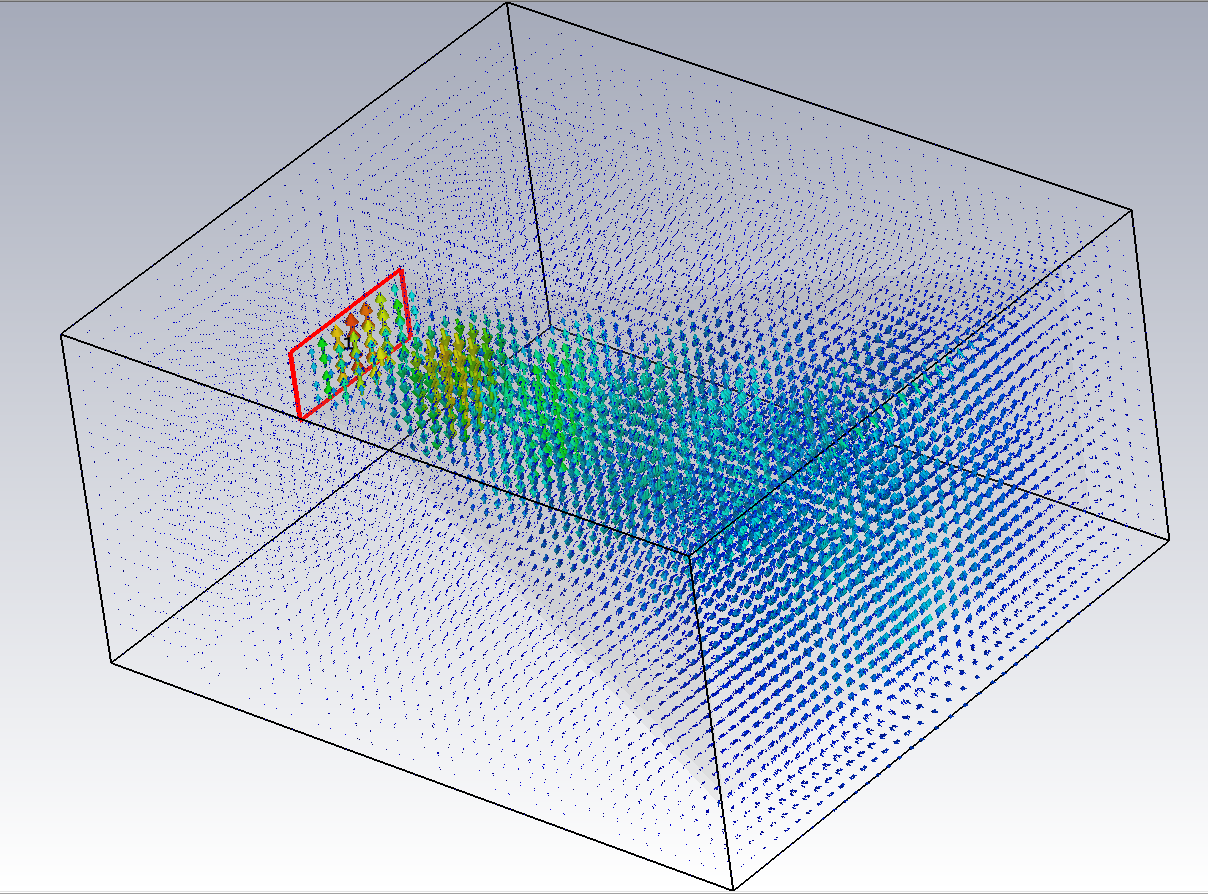
\includegraphics[width=0.8\textwidth]{18.png}
\end{figure}

\textbf{波导口电场：} 在 10.3 GHz 工作频率下，波导端口处电场呈现清晰的 TE10 模分布特征，电场方向垂直于波导宽边，中心场强最大，向两侧递减。

\textbf{喇叭口电场：} 在喇叭口径面上，电场分布由波导口的 TE10 模平滑过渡为近似均匀分布，整个口径面场强较为一致。这种分布有助于将电磁能量有效地辐射到自由空间，并形成良好的定向方向图。

\textbf{电场传播过程：} 电场分布图完整展示了电磁波从波导口经喇叭过渡段到口径面的演变过程，验证了喇叭天线对波导与自由空间进行阻抗匹配的核心作用。

\section*{三、实验收获与体会}

通过本次 CST 仿真实验，我掌握了矩形波导馈电角锥喇叭天线的完整建模与仿真流程，包括参数化建模、Loft 放样、Shell 掏空、端口设置、边界条件设置等操作。同时，我学会了如何分析天线的 S11 参数、VSWR、方向图和增益等关键性能指标。实验中遇到的操作问题（如命令位置变化、Loft 无法激活等）也锻炼了我查阅资料和解决问题的能力。本实验加深了我对喇叭天线工作原理和口径天线辐射特性的理解。

\end{document}